\begin{enumerate}
	\item Draw a circle of radius $3.5 cm$. Take a point $P$ outside the circle at a distance of $7 cm$ from the centre of the circle and construct a pair of tangents to the circle from that point.
	\item Contruct a $\triangle ABC $ with sides $BC = 6 cm$, $AB = 5 cm$ and $\angle ABC = 60\degree$. Then construct a triangle whose sides are $\frac{3}{4}$ of the corresponding sides of $\triangle ABC$.
	\item In \figref{fig:Construction-1.jpg}, $DE \parallel BC $. If $\frac{AD}{DB}=\frac{3}{2}$ and $AE = 2.7 cm$, then $EC$ is equal to
		\begin{enumerate}
		\item $2.0 cm$ 
                \item $1.8 cm$
		\item $4.0 cm$
		\item $2.7 cm$
		\end{enumerate}
		\begin{figure}[!ht]
			\begin{center}
				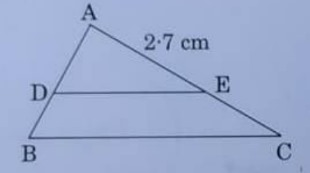
\includegraphics[width=\columnwidth]{figs/Construction-1.jpg}
			\end{center}
			\caption{}
			\label{fig:Construction-1.jpg}
		\end{figure}
		\newpage
	\item In \figref{fig:Construction-2.jpg}, if $PQ \parallel BC$ and $PR \parallel CD$ that $\frac{QB}{AQ} = \frac{DR}{AR}$.



		\begin{figure}[!ht]
			\begin{center}
				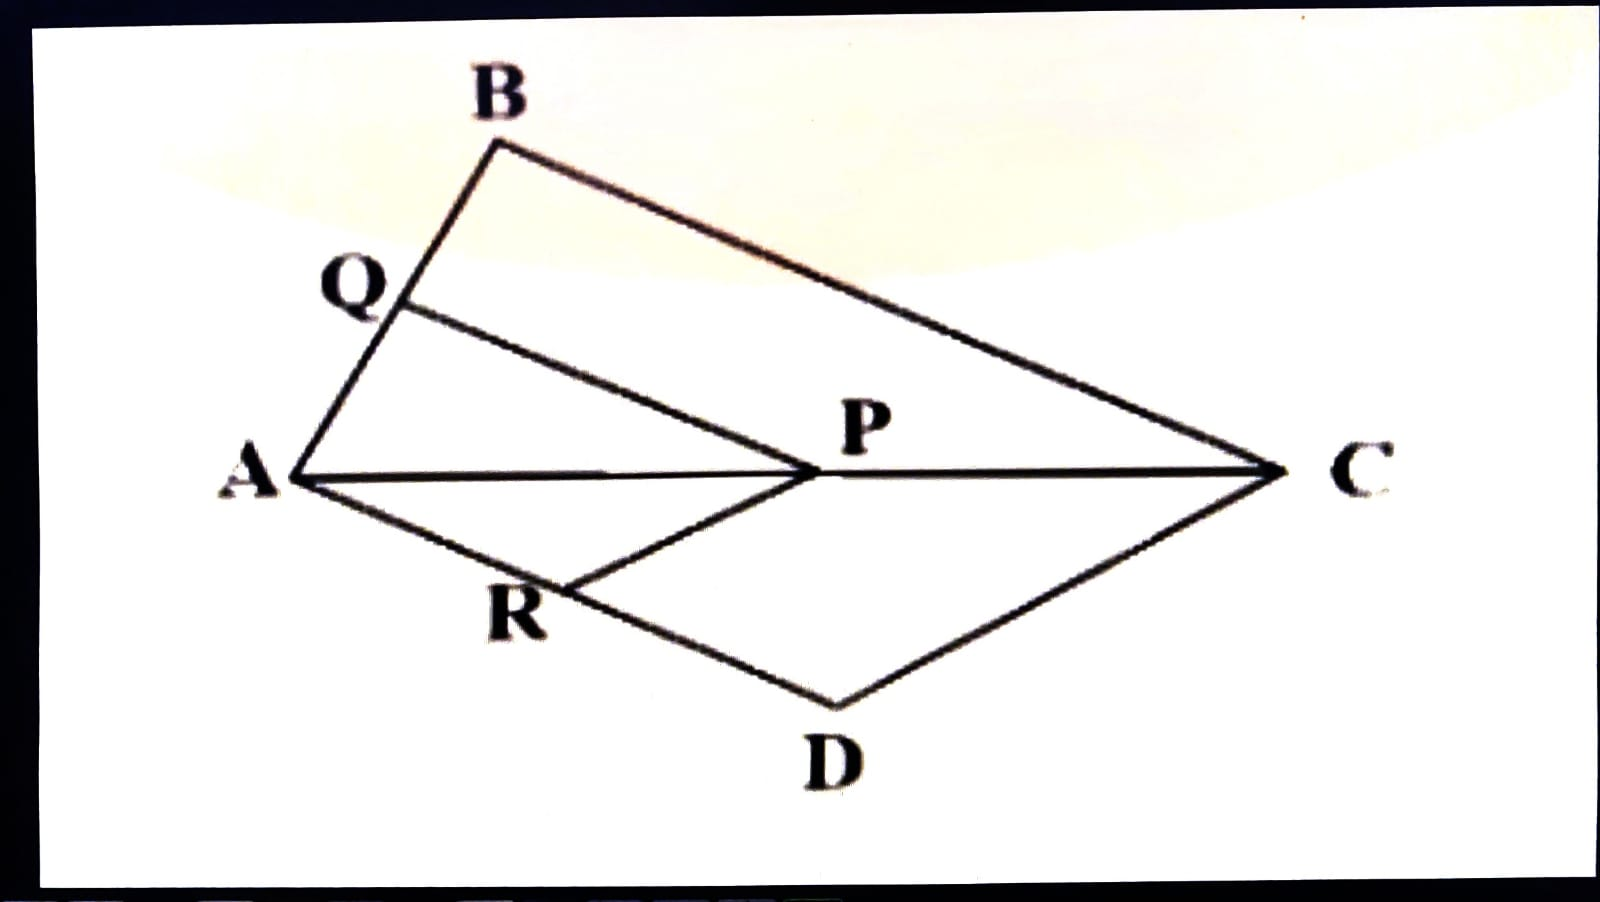
\includegraphics[width=\columnwidth]{figs/Construction-2.jpg}
			\end{center}
			\caption{}
			\label{fig:Construction-2.jpg}
		\end{figure}
\end{enumerate}

